\documentclass[11pt, a4paper]{article}
%\usepackage{proj1}
\usepackage{natbib}
\usepackage{fancyhdr}  
\usepackage{subcaption}
\usepackage{caption}
\usepackage{graphicx}
\linespread{1.25} 
\setlength{\parindent}{0cm}
\graphicspath{{Images/}}
\usepackage{hyperref}
\usepackage{amsmath}
\usepackage{amsfonts}
\usepackage{amssymb}
\usepackage{amsthm}
\usepackage{mathtools}
\usepackage{commath}

%\usepackage[sc,osf]{mathpazo}
\usepackage{subcaption}
\usepackage[a4paper, top=1in, left=1.0in, right=1.0in, bottom=1in, includehead, includefoot]{geometry} %Usually have top as 1in

\usepackage{listings}
\usepackage{color} %red, green, blue, yellow, cyan, magenta, black, white
\definecolor{mygreen}{RGB}{28,172,0} % color values Red, Green, Blue
\definecolor{mylilas}{RGB}{170,55,241}


\hypersetup{colorlinks,linkcolor={black},citecolor={blue},urlcolor={black}}
\usepackage{color}
\urlstyle{same}


\theoremstyle{definition}
\newtheorem{definition}{Definition}[section]

\title{Exact Solutions for the Full Problem \\with Force Control and with Flow Control}
\date{}
\newcommand{\Sta}{\rho}
\newcommand{\Adj}{p}
\newcommand{\Con}{u}

\pagenumbering{gobble}
\begin{document}
	\section{2D Example 1}
	We choose $\rho_0 = 0.25$ and
	\begin{align*}
	\hat \rho = 0.25(1-t) + t\frac{1}{4}((\cos(\pi y_1)+1)(\cos(\pi y_2)+1)),  
	\end{align*}
	as in last week's report. Note the control plots were wrong. Now below the correct ones. The four Figures \ref{Control1},\ref{Control2}, \ref{Control3} and \ref{Control4} show the optimal control for different parameters. The number of points is very small: $n=10$, $N =20$, but larger examples are running on the server.\\
	For forward and optimal $\rho$ the following results are copied in from last week as a reminder (with larger number of points):
	We choose $n = 20$, $N_1,N_2 = 30$. Tolerances are $10^{-8}/10^{-4}$.
	For $\beta = 10^{-3}$ and $\gamma = 1$, $J_{FW} = 0.0596$ and $J_{Opt} = 0.0170$, see \ref{Fig2D1}, \ref{Fig2D2}.
	For $\beta = 10^{-3}$ and $\gamma = -1$, $J_{FW} = 0.0334$ and $J_{Opt} = 0.0020$, see \ref{Fig2D4}, \ref{Fig2D5}.
	\\
	\\
	Code for flux plots. Correct?
	\begin{align*}
	&PlotArea.NFlux = 30;\\
	&PlotArea.y1Min = -1;\\
	&PlotArea.y1Max = 1;\\
	&PlotArea.y2Min = -1;\\
	&PlotArea.y2Max = 1;\\
	&output1a.IDC.InterpolationPlotFlux(PlotArea)\\
	&flnorm = max(max(abs(output1a.OptimizationResult.Control)));\\
	&fl = Control(ti,:)';\\
	&maskAdd = fl > 10^-3;\\
	&output.IDC.plotFlux(fl,maskAdd,flnorm,1.2,'k',false,0);\\
	&output.IDC.plotStreamlines(fl,[],[],[]);	
	\end{align*}
	
	\begin{figure}[h]
		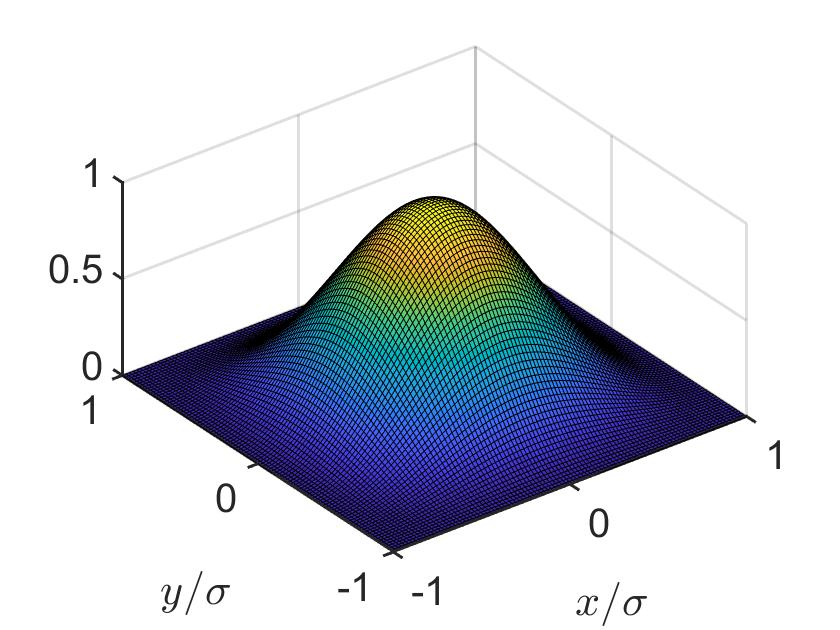
\includegraphics[scale=0.3]{rhoHat2D1.jpg}
		\caption{2D Example 1, $\hat \rho$ at $t=T$}
		\label{rhoHat2d1}
	\end{figure}
	
	\begin{figure}[h]
		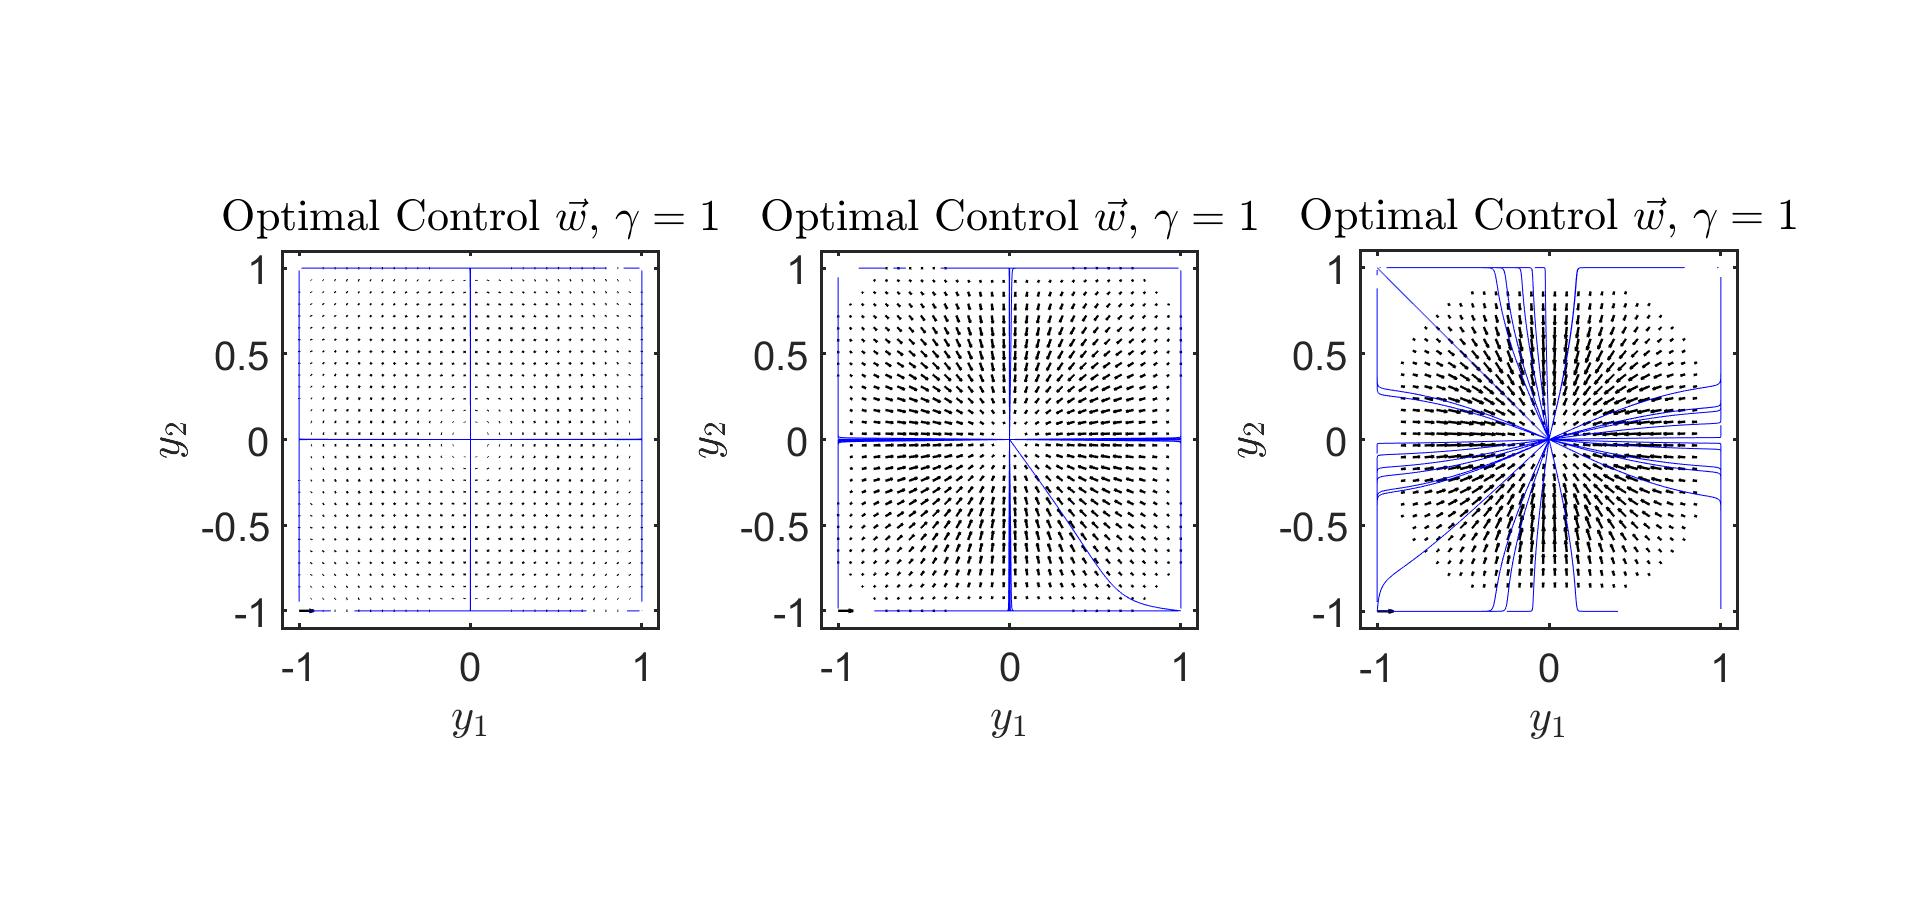
\includegraphics[scale=0.25]{FigC1.jpg}
		\caption{2D Example 1, Control $\gamma = 1$, $\beta = 10^{-3}$, $t = 2,5,9$}
		\label{Control1}
    \end{figure}
	\begin{figure}[h]
		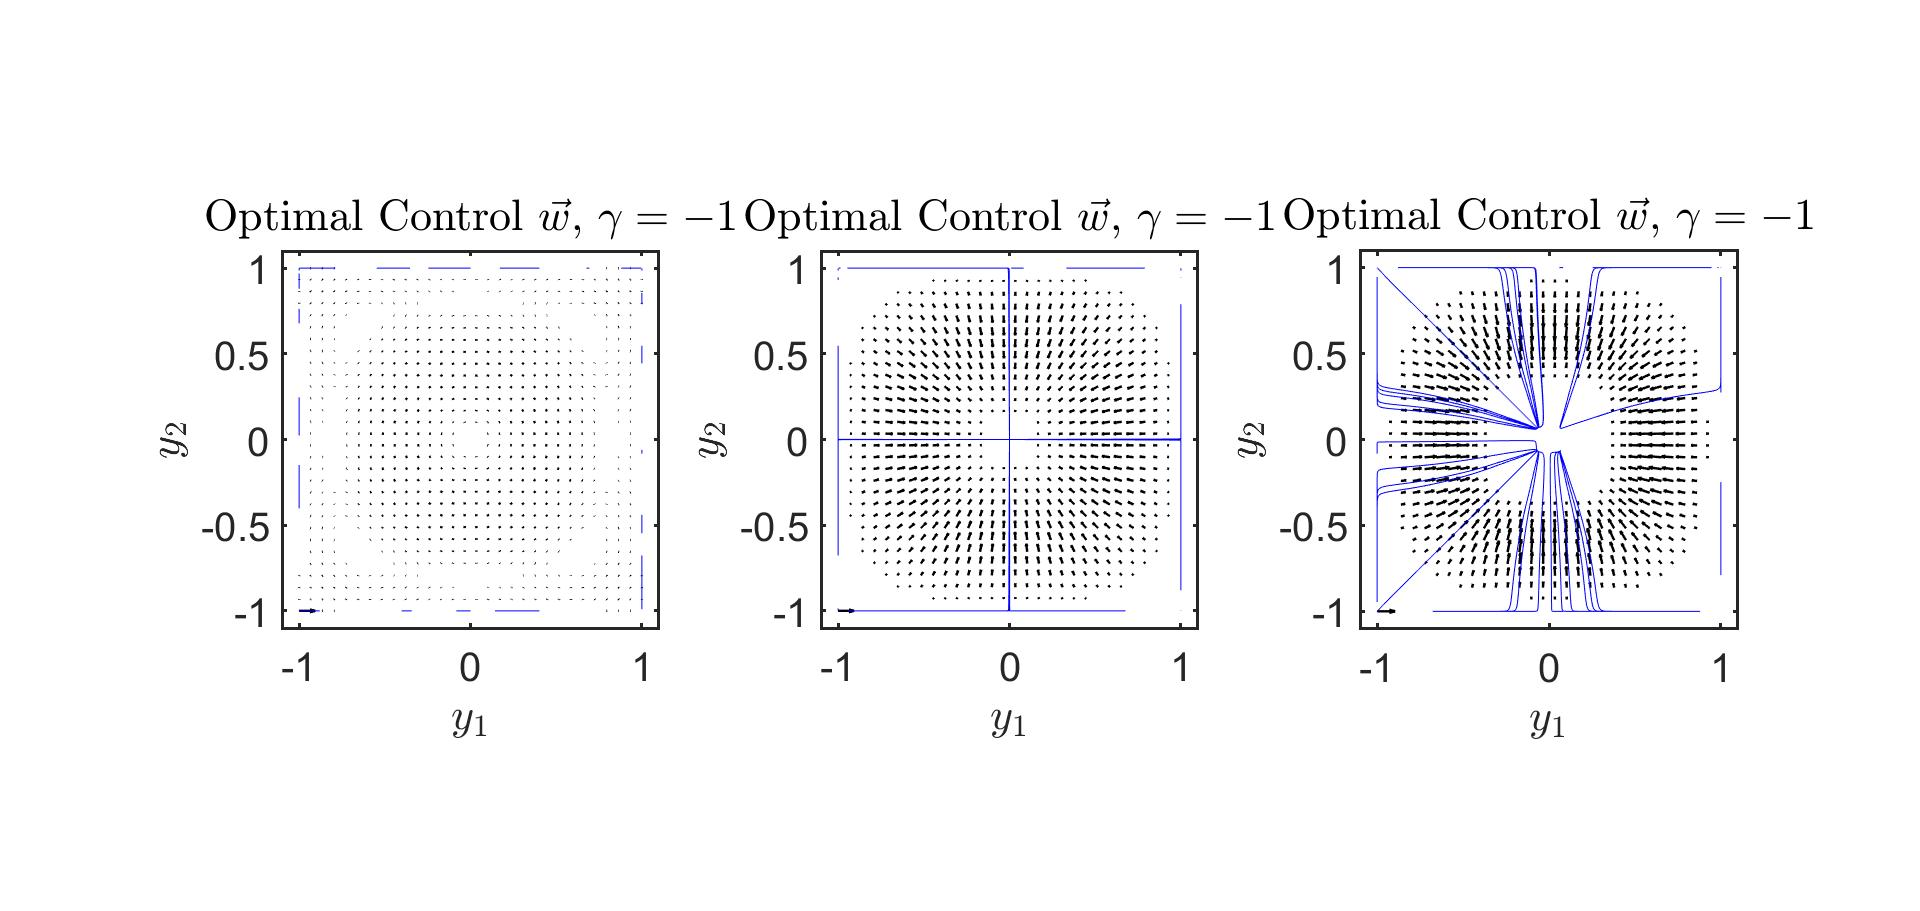
\includegraphics[scale=0.25]{FigC2.jpg}
		\caption{2D Example 1, Control $\gamma = - 1$, $\beta = 10^{-3}$, $t = 2,5,9$}
		\label{Control2}
	\end{figure}
	\begin{figure}[h]
		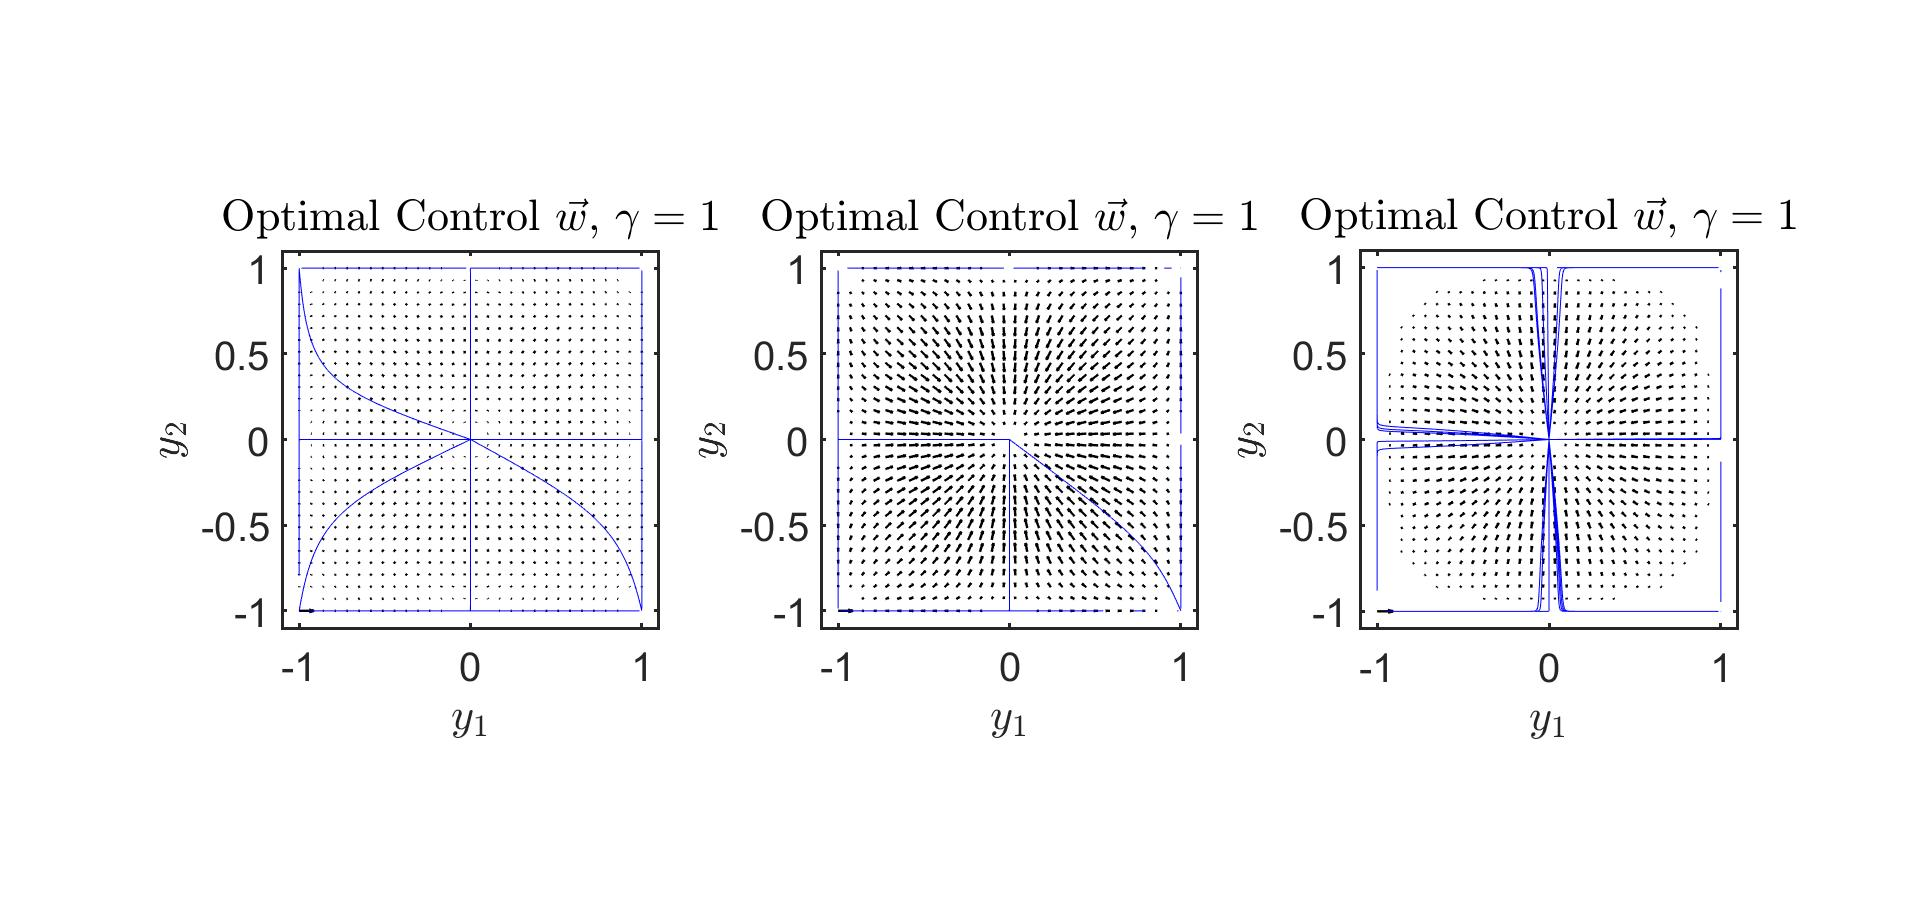
\includegraphics[scale=0.25]{FigC3.jpg}
		\caption{2D Example 1, Control $\gamma = 1$, $\beta = 10^{-1}$, $t = 2,5,9$}
		\label{Control3}
	\end{figure}
	\begin{figure}[h]
		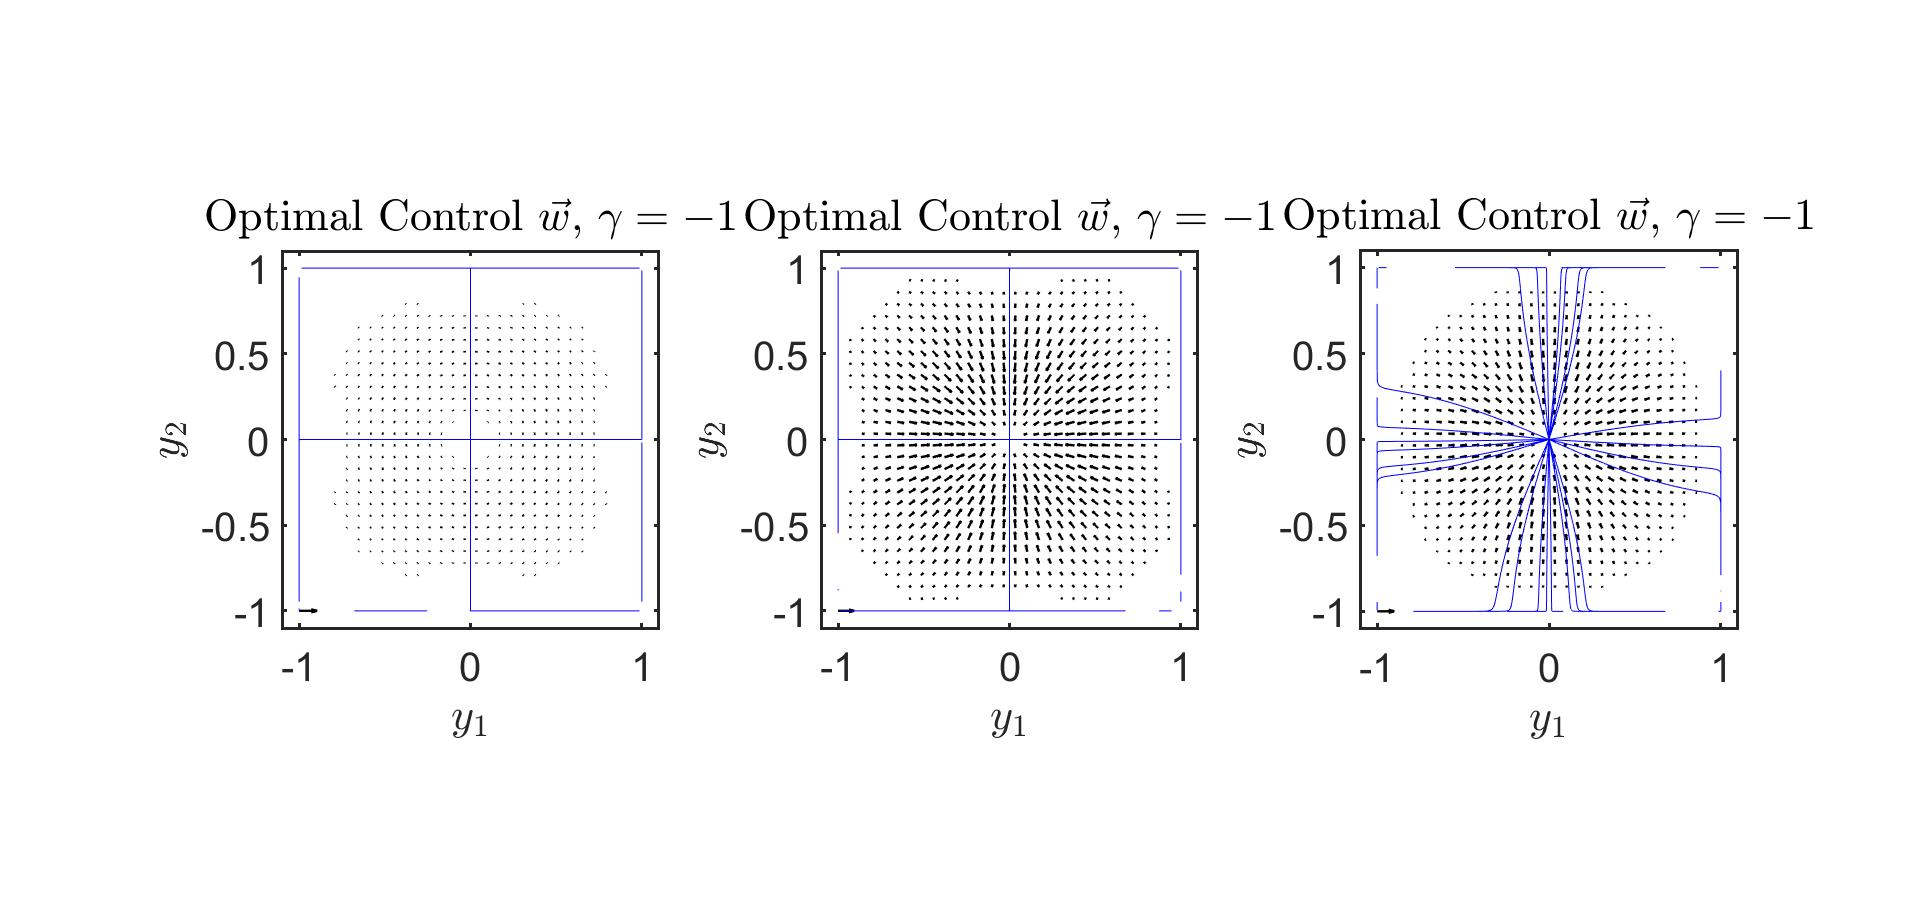
\includegraphics[scale=0.25]{FigC4.jpg}
		\caption{2D Example 1, Control $\gamma = -1$, $\beta = 10^{-1}$, $t = 2,5,9$}
		\label{Control4}
	\end{figure}
	
	
	
	\begin{figure}[h]
		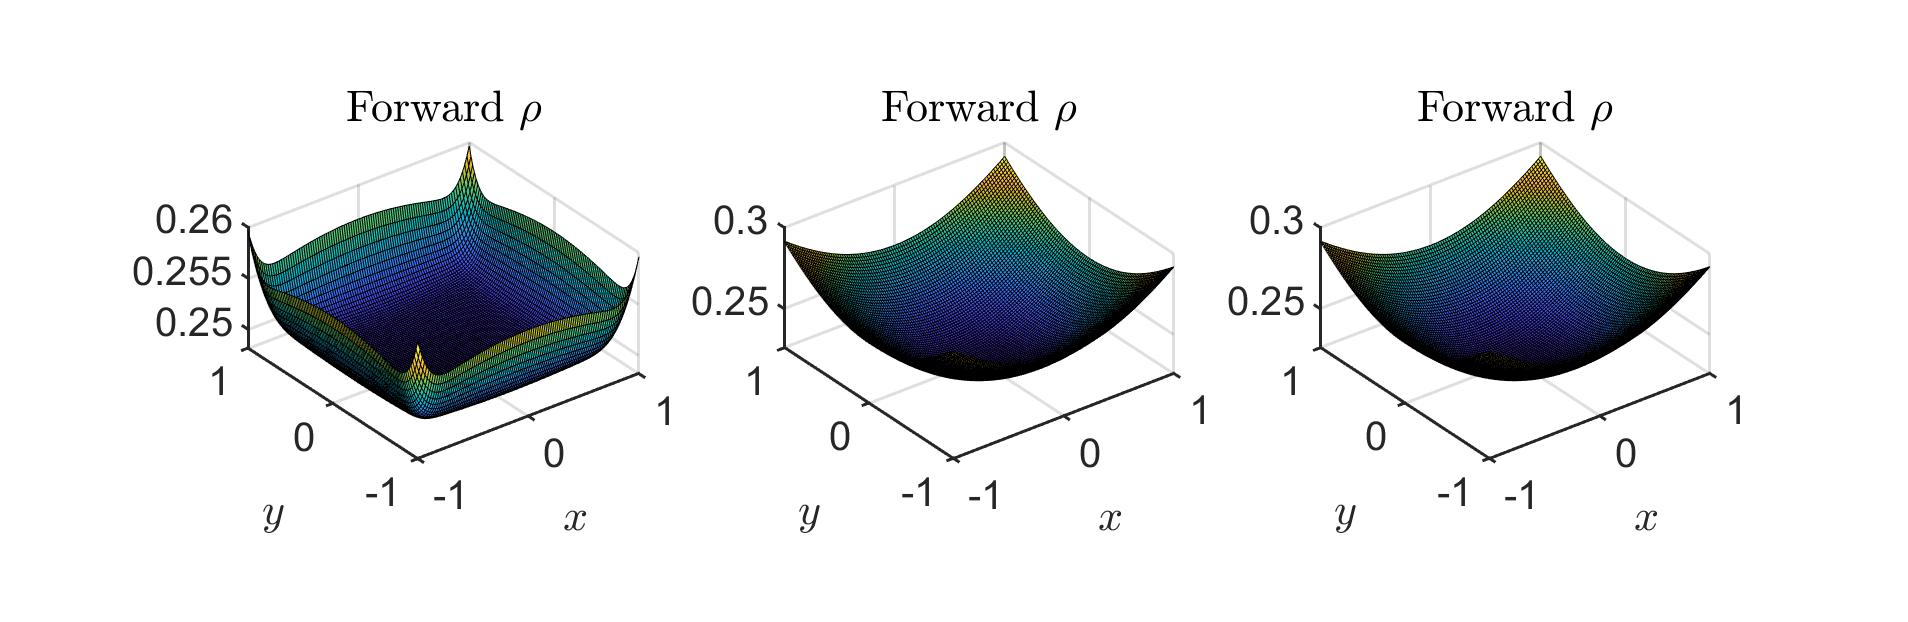
\includegraphics[scale=0.25]{FWrho2Dg1.jpg}
		\caption{2D Example 1, $\rho$ forward, $t= 2,10,20$, $\beta = 10^{-3}$, $\gamma = 1$}
		\label{Fig2D1}
	\end{figure}
	\begin{figure}[h]
		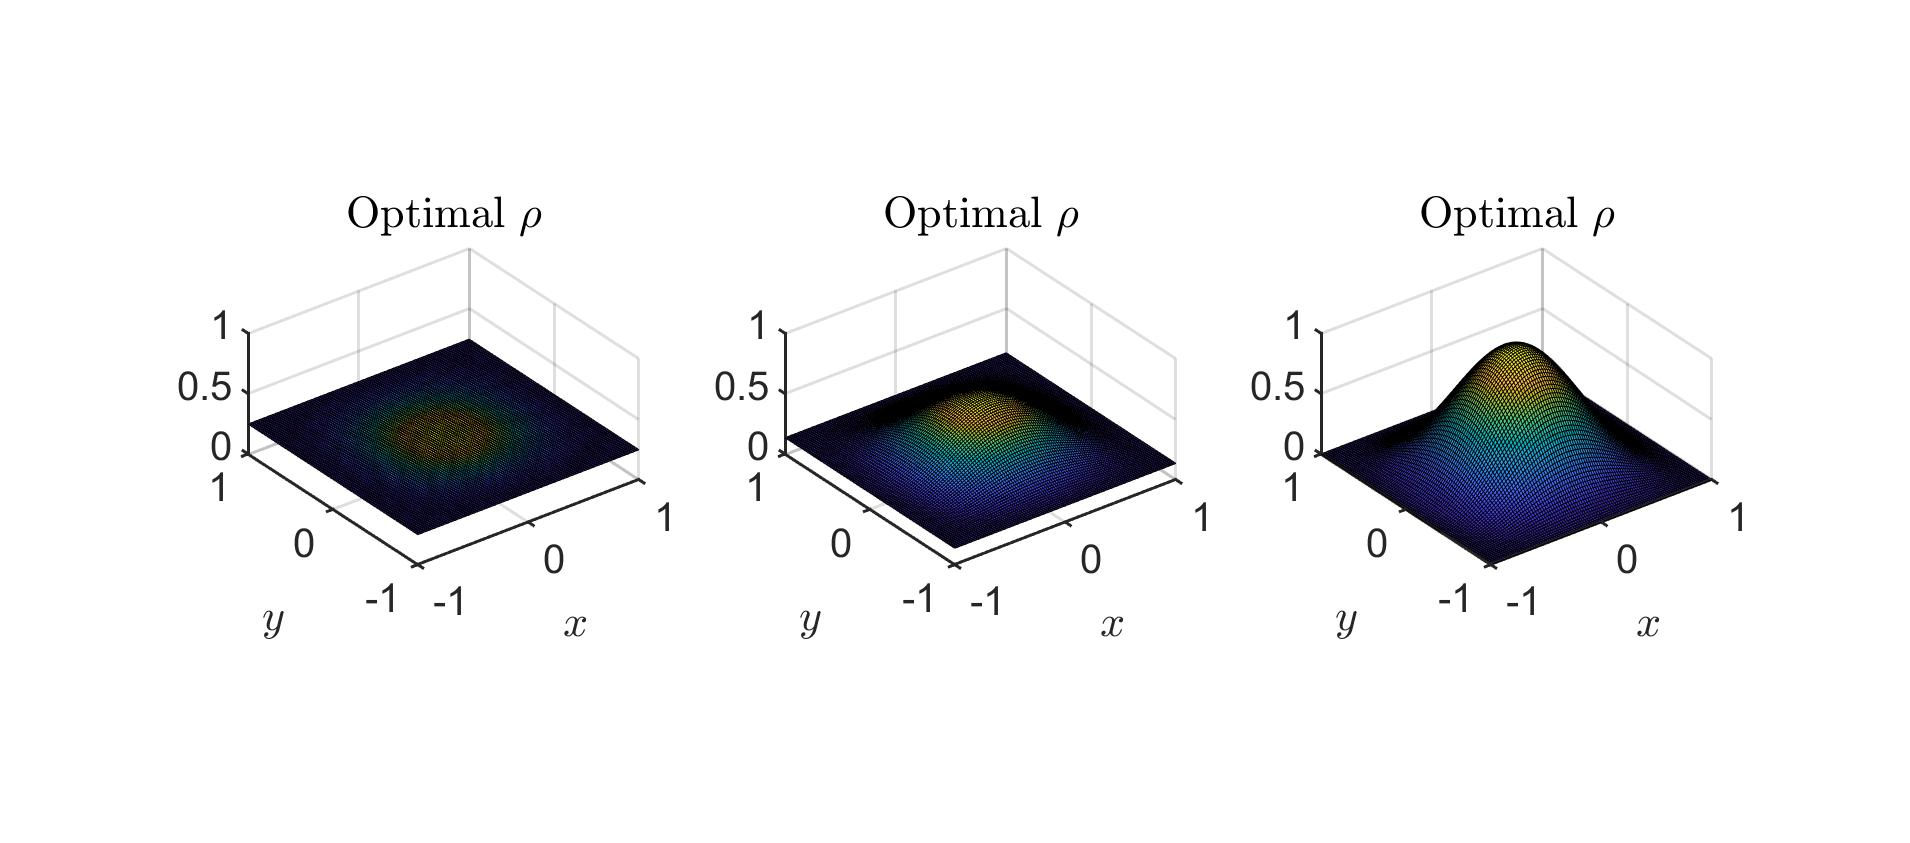
\includegraphics[scale=0.25]{Optrho2Dg1.jpg}
		\caption{2D Example 1, $\rho$ optimal, $t= 2,10,20$, $\beta = 10^{-3}$, $\gamma = 1$}
		\label{Fig2D2}
	\end{figure}
	\begin{figure}[h]
		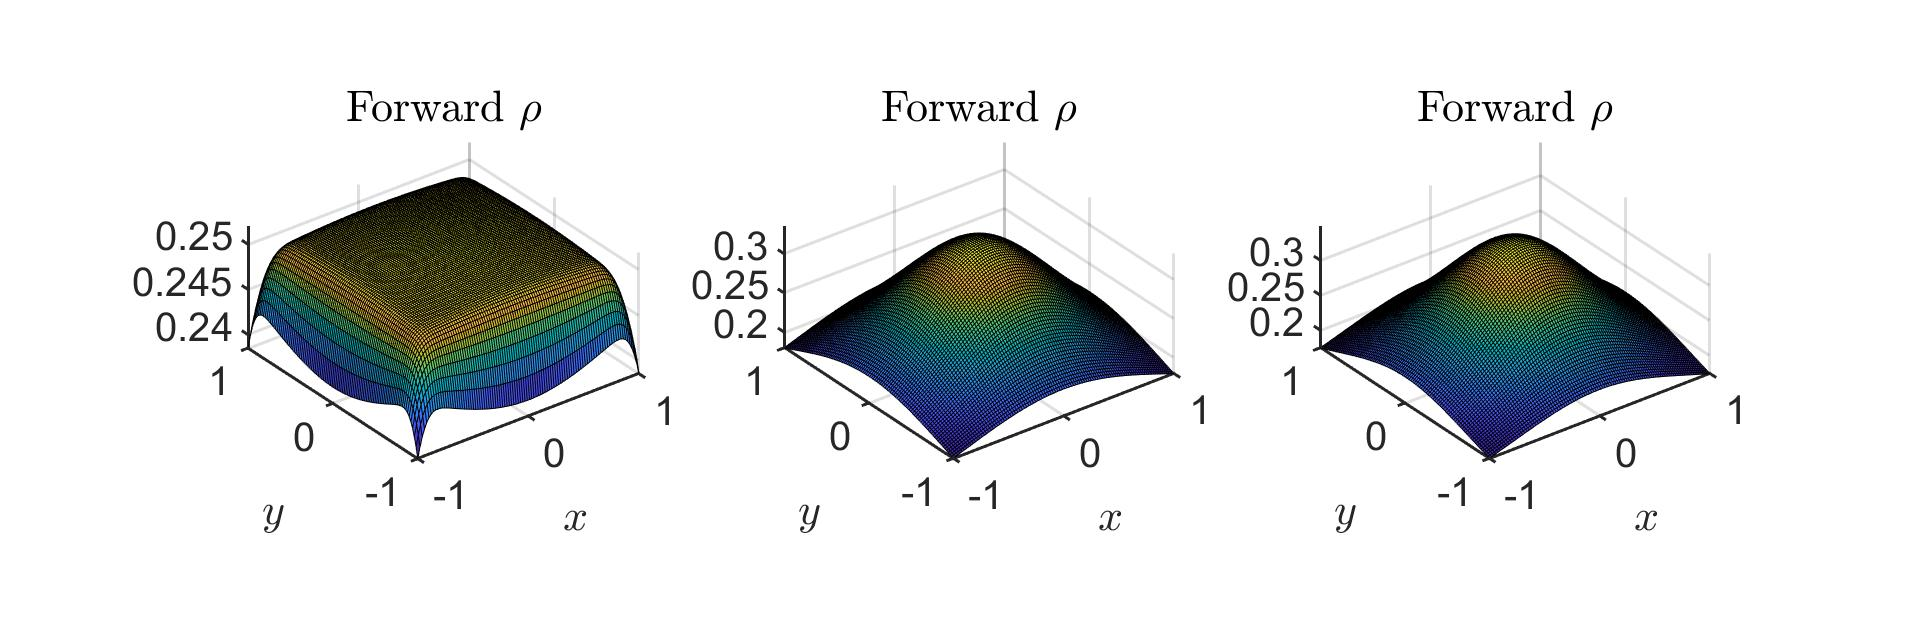
\includegraphics[scale=0.25]{FWrho2Dgn1.jpg}
		\caption{2D Example 1, $\rho$ forward, $t= 2,10,20$, $\beta = 10^{-3}$, $\gamma = -1$}
		\label{Fig2D4}
	\end{figure}
	\begin{figure}[h]
		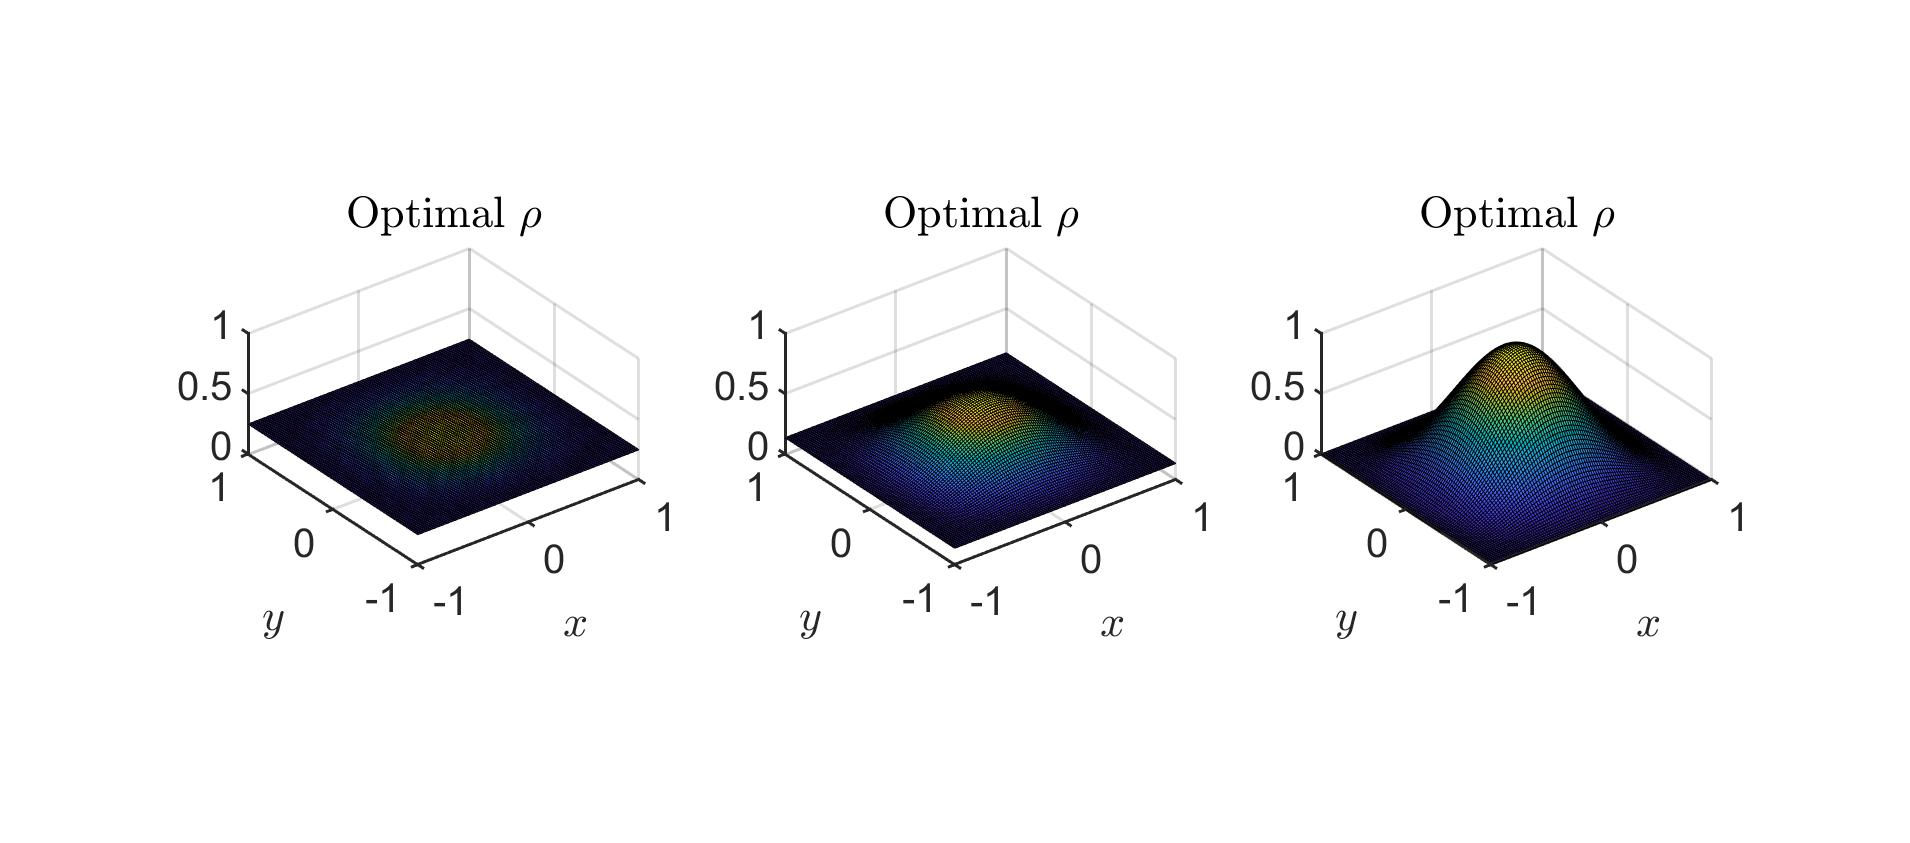
\includegraphics[scale=0.25]{Optrho2Dgn1.jpg}
		\caption{2D Example 1, $\rho$ optimal, $t= 2,10,20$, $\beta = 10^{-3}$, $\gamma = -1$}
		\label{Fig2D5}
	\end{figure}
	
	
\end{document}